\chapter{Derived Schema of Symmetric Crypto}

\section{SHA3 Derived Schemes}
\begin{flushleft}

    Abbiamo detto che una funzione hash ritorna come output una quantità fissa di bytes. Se quindi ci dovesse essere la necessità di avere \textbf{meno dati}, allora ``basterebbe'' \textbf{troncare} il \textbf{\textit{digest}}, nel caso opposto invece possiamo ri-progettare un algoritmo simile a \textbf{CTR} e invocarlo più volte, il che, però, porterebbe molto più sforzo da parte degli sviluppatori e rischierebbe di introdurre delle vulnerabilità nel codice.
    
    \smallskip

    È stato quindi introdotto il \textbf{\textit{eXtendible Output Function - XOF}} ovvero una \textbf{\textit{variable-length hash funciton}}.

    \smallskip

    \textcolor{red}{\textbf{\textit{cSHAKE}}}: è una variante di SHA3 e accetta i seguenti input addizionali:
    \begin{enumerate}[nosep]
        \item \textbf{\textit{output length}}: definisce la dimensione del digest.
        \item \textbf{\textit{custom string}}: specializza l'esecuzione della funzione \textit{hash} per un certo \textbf{contesto}. È molto utile per \textbf{\textit{domain (contest) separation}}.
    \end{enumerate}

    \begin{figure}[h]
        \centering
        \begin{minipage}[c]{0.45\textwidth}
            \textbf{cSHAKE128} ha 128bit di sicurezza ed è una variante di SHA3-256.
        \end{minipage}
        \hfill
        \begin{minipage}[c]{0.45\textwidth}
            \textbf{cSHAKE256} ha 256bit di sicurezza ed è una variante di SHA3-512.
        \end{minipage}
    \end{figure}

    \smallskip

    \textcolor{red}{\textbf{\textit{TupleHash}}}: è una funzione \textit{hash} ha delle interfacce con un astrazione \textit{high-level}, infatti permette di accettare una \textbf{lista di valori} e una \textbf{\textit{custom string}} come input. È un \textit{wrap} di \textbf{cSHAKE} che permette di supportare delle liste come valore di input, alle quali viene prima applicata una codifica in modo non ambiguo assegnando ad ogni elemento un'unica sequenza di bit - bitstring - poi verrà passata a cSHAKE come input. La \textit{custom string} ha un valore di default al quele viene concatenato quello dell'utente: \textit{TupleHash}. È utilizzata per evitare ambiguità di concatenazione. È deterministica e strutturate, utile in contesti crittografici dove serve un hash sicura su strutture dati complesse.

    \smallskip

    \textcolor{red}{\textbf{\textit{ParallelHash}}}: è progettato per per sfruttare ambienti paralleli (multi-core, GPU, ecc.) allo scopo di accelerare il calcolo dell'hash su grandi quantità di dati.
    \begin{enumerate}[nosep]
        \item i dati vengono suddivisi in blocchi.
        \item per ogni blocco viene calcolato il \textit{digest} in parallelo.
        \item i \textit{digest} dei vari blocchi (\textbf{\textit{digest parziali}}) vengono poi combinati per calcolare un \textit{digest} finale sugli output precedenti, ottenendo il digest complessivo del messaggio.
    \end{enumerate}
    Questo approccio ricorda un \textbf{\textit{Merkle Hash Tree - MHT}} dove le foglie sono gli hash dei blocchi e il nodo radice è l'hash finale ottenuto dall'unione degli hash sottostanti. \\ 
    \textbf{\textit{N.B.}} esistono funzioni di hash - ad esempio \textbf{Blake2} - che hanno meccanismi interni che la rendono automaticamente parallelizzabili anche senza un architettura come quella di ParallelHash.

    \smallskip

    \textcolor{red}{\textbf{\textit{MAC for SHA3}}}: \textbf{SHA3} è stato progettato e sviluppato per evitare \textbf{\textit{length extesion attack}} è quindi possibile non utilizzare l'\textbf{HMAC} basato su SHA3, in quanto ci sarebbe dell'\textit{overhead} inutile, ma sarebbe possibile avere un MAC che si basa su SHA3 come:

    {\centering
        \textbf{tag} $\leftarrow$ \textcolor{red}{\textbf{SHA3(k || message)}}
    \par}

    Bisogna solo fare attenzione a non utilizzare questo metodo con funzioni di hash che utilizzano come primitiva la costruzione \textbf{Merkle-Damgard} - per SHA2 utilizzare HMAC.

    \smallskip

    \textcolor{red}{\textbf{\textit{KMAC}}}: è un \textbf{MAC} a dimensione variabile che si basa su \textbf{cSHAKE}. Come input \textbf{KMAC} richiede:
    \begin{enumerate}[nosep]
        \item una \textbf{chiave} segreta $k$.
        \item un \textbf{messaggio} $m$.
        \item una \textbf{\textit{custom string}} che verrà concatenato al valore di default \textit{KMAC}.
        \item una \textbf{lunghezza} desiderata dell'output.
    \end{enumerate}
    Vengono combinati, in maniera sicura, la chiave, il messaggio e la \textit{custom string}, il tutto viene passato in input a cSHAKE che ne calcola il \textbf{tag}.

    \begin{figure}[h]
        \centering
        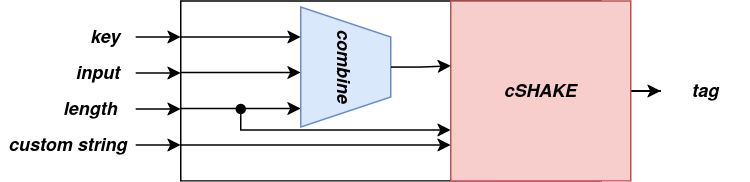
\includegraphics[width=0.75\textwidth]{img/kmac.png}
    \end{figure}
\end{flushleft}

\newpage

\section{Key Derivation Function}

\begin{flushleft}
    Molti schemi crittografici e protocolli spesso richiedono almeno due chiavi segrete non correlate, ma di contro si cerca di dover gestire un'unica chiave durante le procedure di \textit{key management} e di \textit{key distribution}.

    \smallskip

    Le \textbf{\textit{KDF}} sono funzioni che permetto di generare più \textit{pseudo-random keys} partendo da una singola chiave. Le \textbf{KDF} sono simili a delle \textbf{PRF}, infatti, prendono in input una singola stringa segreta e in maniera \textbf{deterministica} in output verrà generata una sequenza più lunga di dati pseudo-random che possono essere utilizzate come chiavi indipendenti e multiple. A differenza dei \textbf{PRF}, però, la \textbf{KDF} è progettata per generare una sequenza più corta e in più possono supportare altre funzionalità - ad esempio \textbf{\textit{input string}}, \textbf{\textit{explicit salting}} e lo \textbf{\textit{scoping}}. \\
    È possibile re-implementare una \textbf{KDF} utilizzando come primitive \textit{block cipher}, \textit{stream cipher}, MAC o \textit{hash function}. Esistono, però, delle \textbf{KDF} stardandizzate dal NIST, la più popolare è chiamata \textbf{HKDF} e si basa su un \textbf{HMAC}.

    \smallskip

    Un'implementazione di alto livello di una \textbf{KDF} ha due funzioni interne:
    \begin{enumerate}[nosep]
        \item \textcolor{red}{\textbf{\textit{extraction}}}: che dato una \textit{secret string} - possibilmente \textbf{non uniforme} e con un \textbf{alto livello di entropia} (comparabile con il \textit{security level}) - genera \textbf{una} chiave segreta (pseudo-random) uniforme.
        \item \textcolor{blue}{\textbf{\textit{expansion}}}: data una \textit{secret key} uniforme genera una chiave \textbf{pseudorandom} più lunga - ad esempio generare una chiave da un'altra per \textit{key scoping} o \textit{key rotation}
    \end{enumerate}

    \begin{figure}[h]
        \centering
        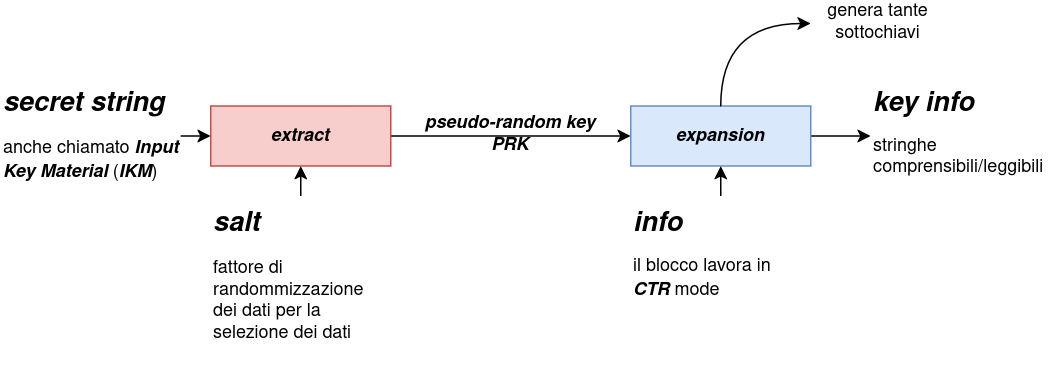
\includegraphics[width=\textwidth]{img/kdf.png}
    \end{figure}

    Una \textbf{KDF} è un metodo sicuro per derivare una chiave segreta anche se l'input è una string non uniforme (uniforme = alta entropia), ma l'input deve avere alta entropia e, ad esempio, una password per definizione - segreto che può essere ricordato da un umano - raramente ha abbastanza entropia $\rightarrow$ \textbf{\textit{Password-Based Key Derivation}} anche note come \textbf{\textit{Password Hashing}}. Nel caso in cui si abbia già un segreto random binario possiamo \textit{bypassare} il blocco di \textbf{\textit{extract}} e passare subito all'\textbf{\textit{expansion}}. Una \textbf{KDF} può dare funzionalità aggiuntive tra cui: aggiungere \textbf{randomicità} e aggiungere \textit{scoping information} (ad esempio per fare \textit{domain separation}).

    \smallskip

    Gli input di una \textbf{HKDF} sono:
    \begin{itemize}[nosep]
        \item l'\textbf{algoritmo}: la funzione di hash interna (SHA256).
        \item \textbf{\textit{string}}: è la stringa segreta (con alta entropia).
        \item \textbf{\textit{length}}: lunghezza desiderata per la chiave derivata - simile all'input della dimensione per \textbf{XOF} e \textbf{KMAC}.
        \item \textbf{\textit{info}}: è una stringa che rappresenta il contesto per la separazione dei domini.
        \item \textbf{\textit{salt}}: è una stringa, è opzionale, se viene utilizzata normalmente è una stringa randomica con lunghezza compatibile con la dimensione dell'algoritmo di hash utilizzato per l'\textbf{HMAC}
    \end{itemize}
    L'output è una \textbf{chiave pseudorandom} di dimensione \textbf{\textit{length}}.
    L'\textbf{HKDF} include due sottofunzioni (che vengono spesse esposte dalle librerie crittografiche):
    \begin{itemize}[nosep]
        \item \textbf{HKDF-Extract}: dato un \textbf{IKM} ritorna una chiave pseudo-random \textbf{PRK} di dimensione \textbf{\textit{alg.digest\_size}}
        \item \textbf{HKDF-Expand}: dato un \textbf{PRK} ritorna una chiave pseudo-random $\mathbf{key_{info}}$ di dimensione \textbf{\textit{length}}
    \end{itemize}
    \textcolor{orange}{\textbf{Esempio - PyCryptoDome}}
\end{flushleft}

\begin{lstlisting}[language=python, label={hkdf}]
    # from source code
    def HKDF(master, key_len, salt, hashmod, num_keys=1, context):
        output_len = key_len * num_keys
        if output_len > (255 * hashmod.digest_size):
            raise ValueError("Too much secret data to derive")
        if not salt:
            salt = b'\x00' * hashmod.digest_size
        if context is None: context = b""
        prk = _HKDF_extract(salt, master, hashmod)
        okm = _HKDF_expand(prk, context, output_len, hashmod)
        if num_keys == 1:
            return okm[:key_len]
        kol = [okm[idx:idx + key_len]
            for idx in iter_range(0, output_len, key_len)]
        return list(kol[:num_keys])
\end{lstlisting}

\begin{flushleft}
    \textcolor{red}{\textbf{\textit{HKDF-Extract}}}: trasforma una \textit{key} ad alta entropia in un segreto con distribuzionde di entropia uniforme di dimensione \textbf{hashmod.digest\_size}, può non essere invocata nel caso in cui si abbia già una chiave segreta con distribuzione uniforme e possiamo soltato fare il procedimento di espansione.

    \begin{center}
        \begin{minipage}[t]{0.45\textwidth}
            \textbf{Chiave ad Alta Entropia}: significa che la chiave è imprevedibile, contiene molta ``casualità''. Per esempio, una stringa di 256 bit generata da un generatore casuale crittograficamente sicuro. Tuttavia, non è detto che sia uniforme: alcuni bit potrebbero avere distribuzioni sbilanciate (es. più 1 che 0).
        \end{minipage}
        \hfill
        \begin{minipage}[t]{0.45\textwidth}
            \textbf{Chiave Uniforme}: ogni possibile valore è \textbf{equiprobabile}. Questo è importante per alcune operazioni crittografiche, come l'uso in HMAC, perché riduce il rischio di bias che può compromettere la sicurezza.
        \end{minipage}
    \end{center}

    Normalmente il \textbf{\textit{salt}} può essere utilze per integrare l'\textbf{HKDF} in certi protocolli ed è necessario che sia una stringa uniforme, verrà utilizzata come chiave dell'\textbf{HMAC}.

    \smallskip

    \textcolor{orange}{\textbf{Esempio - PyCryptoDome}}
\end{flushleft}

\begin{lstlisting}[language=python, label={hkdf_extract}, caption={\_HKDF\_extract da PyCryptoDome}]
    # from source code
    def _HKDF_extract(salt, ikm, hashmod):
        # HMAC.new(key, msg=b"", digestmod=None):
        prk = HMAC.new(salt, ikm, digestmod=hashmod).digest()
        return prk
\end{lstlisting}

\begin{flushleft}
    \textcolor{red}{\textbf{\textit{HKDF-Expend}}}: dopo che si è ottenuta la \textit{pseudorandom key \textbf{PRK}} bisogna calcolare tanti \textbf{HMAC} quanti ne servono per ottenere la lunghezza finale di $\mathbf{key_{info}}$, che è pari \textbf{\textit{length}} moltiplicata per il numero di chiavi che si vuole generare. Si può notare in ~\ref{hkdf_expand} che l'\textbf{HMAC} viene richiamata in maniera iterativa similmente alla \textit{counter mode}, dove nel caso dell'\textbf{HKDF} il counter è di dimensione 1 byte, è quindi necessario impostare una lunghezza massima per evitare ripetizioni della generazione della chiave che è pari alla \textbf{dimensione} della funzione di \textbf{\textit{hash}} scelta moltiplicata per le possibili combinazioni di un bytes: 255.

    \begin{center} \begin{math} \begin{cases}
                t_0 = \text{HMAC}(\text{PRK}, \; "" \; || \; \text{info} \; || \; 0, \; \text{hashmod}) \\
                t_1 = \text{HMAC}(\text{PRK}, \; t_0 \; || \; \text{info} \; || \; 1, \; \text{hashmod}) \\
                \vdots \\
                t_{i + 1} = \text{HMAC}(\text{PRK}, \; t_i \; || \; \text{info} \; || \; i, \; \text{hashmod}) \\
    \end{cases} \end{math} \end{center}
    \textcolor{orange}{\textbf{Esempio - PyCryptoDome}}
\end{flushleft}

\begin{lstlisting}[language=python, label={hkdf_expand}, caption={\_HKDF\_expand da PyCryptoDome}]
    # from source code
    def _HKDF_expand(prk, info, L, hashmod):
        t, n, tlen = [b""], 1, 0
        while tlen < L:
            hmac = HMAC.new(prk, t[-1] + info + struct.pack('B', n), digestmod=hashmod)
            t.append(hmac.digest())
            tlen, n = tlen + hashmod.digest_size, n + 1
        okm = b"".join(t)
        return okm[:L]
\end{lstlisting}

\newpage

\section{Hash Table Flooding \& small tag MAC's}

\begin{flushleft}
    \textcolor{red}{\textbf{\textit{Hash Table (Hash Map)}}} \\
    L'insieme delle possibili chiavi è rappresentato dall'\textcolor{red}{insieme universo} $\mathcal{U}$ di dimensione $u$. Ad esempio considerando che una chiave è il ``nome e cognome'' di una persona, l'insieme universo sarà formato da tutte le combinazioni dell'insieme dei nomi $\mathcal{N}$ con quello dei cognomi $\mathcal{C}$: 
    
    {\centering
        $\mathcal{N} \times \mathcal{C} \mapsto \mathcal{U}$
    \par}

    Ma noi avremo bisogno di di memorizzare le chiavi in una struttura dati limitata ad esempio in un vettore $T[0, ..., m - 1]$ di dimensione $m$, detta \textbf{tabella di hash}. Definiamo la funzione \textit{hash} è definita come:

    {\centering
        $h: \; \mathcal{U} \mapsto \{0, 1, ..., m - 1\}$
    \par}

    La coppia chiave valore $\langle k, v \rangle$ viene memorizzata in un vettore nella posizione $h(k)$

    \begin{figure}[h]
        \begin{minipage}[t]{0.45\textwidth}
            \centering
            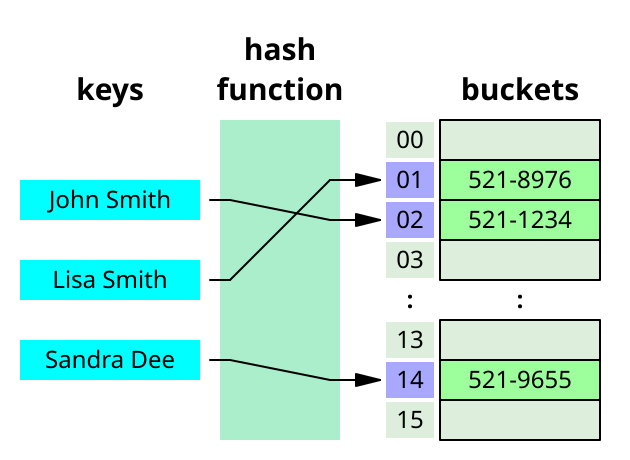
\includegraphics[width=\textwidth]{img/hash_table.png}
        \end{minipage}
        \hfill
        \begin{minipage}[t]{0.45\textwidth}
            \centering
            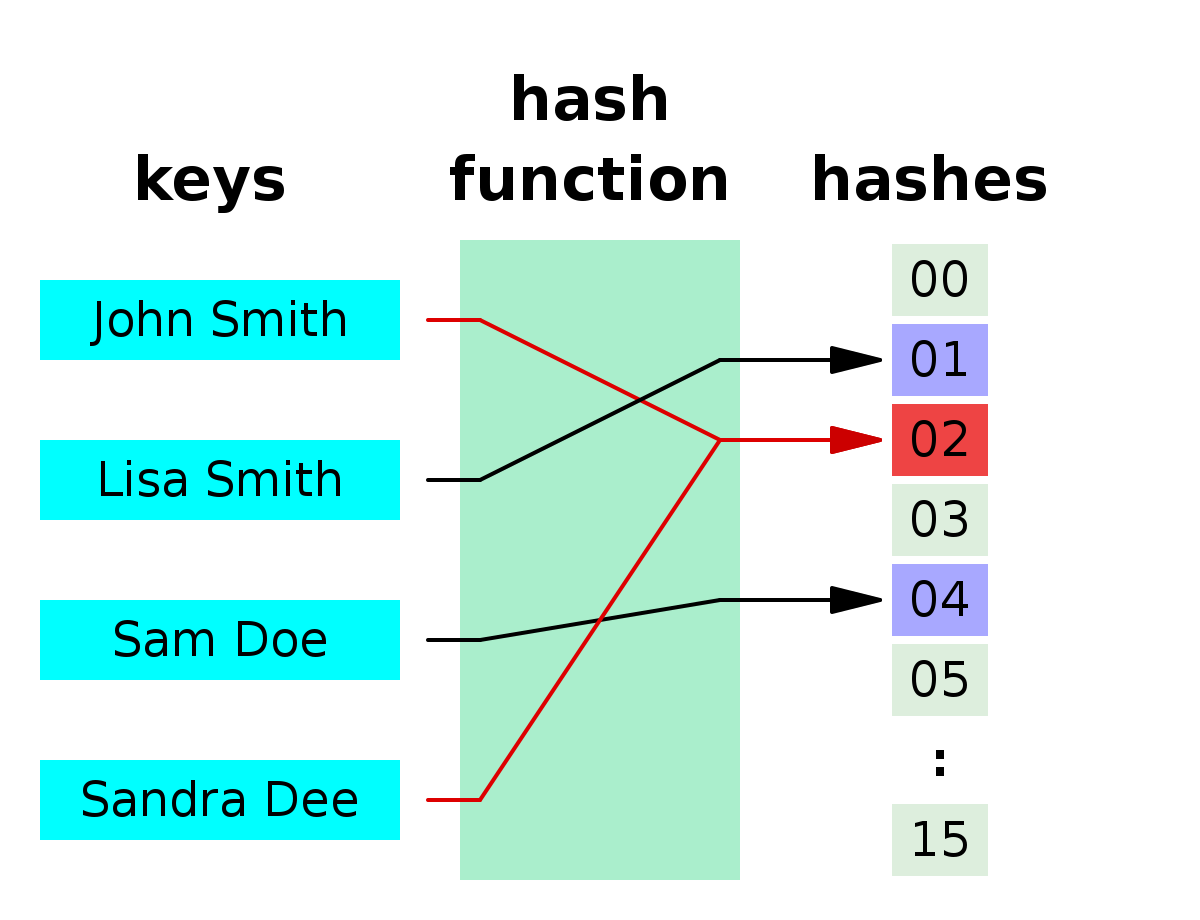
\includegraphics[width=\textwidth]{img/hash_table_coll.png}
        \end{minipage}
    \end{figure}

    L'insieme delle chiavi è potenzialmente infinito, mentre la dimensione della tabella hash non vogliamo che sia infinito - non ho abbastanza memoria. È quindi possibili che ci siano due o più chiavi del dizionario che abbiamo la stessa immagine all'interno della \textbf{tabella di hash}, in questo caso diremo che è avvenuta una collisione. Idealmente vorremo evitarle.

    \smallskip

    Andiamo ora ad analizzare la \textbf{funzione hash} - una funzione hash $h$ si dice \textbf{perfetta} se è \textbf{iniettiva}, ovvero se non da origine a collisioni: $\forall \; k_1, k_2 \in \mathcal{U} \; | \; k_1 \neq k_2 \Rightarrow h(k_1) \neq h(k_2)$ -, differenziando in base alla cardinalità dell'insieme $\mathcal{U}$:
    \begin{itemize}[nosep]
        \item \textbf{tabelle ad accesso diretto}: nel caso in cui $\mathcal{U} \subset \mathbb{Z}^+$ andremo ad utilizzare quella che viene definita \textbf{funzione hash identità} $h(k) = k$. Ad esempio se dobbiamo mappare l'insieme dei pokemon di kanto, numerati da 1 a 151.
    \end{itemize}
    Cerchiamo una funzione che \textbf{distribuiscano uniformemente} le chiavi negli indici $[0, ..., m - 1]$ della tabella hash. \\
    Assunzione: le chiavi possono essere tradotte in valori numerici, anche interpretando la loro rappresentazione in memoria come un numero (python: ord, bin, int). Una delle possibili funzioni possibile è il \textbf{metodo della moltiplicazione di knuth}:

    {\centering
        \begin{minipage}[t]{0.45\textwidth}
            \textbf{Teoria} \\
            m qualsiasi, meglio se potenza di 2 \\ 
            C costante reale, $0 < C < 1$ \\
            sia $i = int(k)$ \\
            $H(k) = \lfloor m (C \cdot i - \lfloor C \cdot i \rfloor) \rfloor$
        \end{minipage}
        \hfill
        \begin{minipage}[t]{0.45\textwidth}
            \textbf{Implementazione} \\
            scelto un valore $m = 2^p$ \\
            sia $w$ - ad esempio 64bit - la dimensione in bit della parola di memoria: $i, m \leq 2^w$ \\
            sia $s = \lfloor C \cdot 2^w \rfloor$ \\
            $i \cdot s$ può essere riscritto come $r_1 \cdot 2^w + r_0$, dove $r_1$ contiene la parte intera di $iC$ e $r_0$ contiene la parte frazionaria di $iC$ \\
            si restituiscano i $p$-bit più significativi di $r_0$
        \end{minipage}
    \par}

    \textcolor{red}{\textbf{Gestione collisione}}: siccome la funzione di \textbf{hash} non è totalmente iniettiva è possibile che avvengano delle collisioni, ovvero che due chiavi abbiamo come immagine lo stesso valore, è possibile gestire queste casistiche in due modi differenti:
    \begin{itemize}[nosep]
        \item \textbf{liste di trabocco} (memorizzazione esterna) - anche noto come \textbf{\textit{chaining}}: le chiavi con lo stesso valore hash $h$ vengono memorizzate in una lista monodirezionale o in vettori dinamici.
        \item \textbf{indirizzamento aperto} (memorizzazione interna)
    \end{itemize}
\end{flushleft}

\begin{flushleft}
    \textcolor{red}{\textbf{Denial of Service via Hash Collision}}: consideriamo una tabella hash, che sfrutta una tabella hash per distribuire i dati su più \textit{bucket}, avremo una ricerca molto efficente (costo costante), ma solamente finché i dati sono distribuiti uniformemente. Si analizzi il caso in cui sia un \textbf{avversario} a scegliere il messaggio e supponiamo sia in grado di generare in maniera efficente un numero elevato di messaggi $m$ tale che $M = \{m \; | \; j = \text{Hash}(m)\}$

    \begin{figure}[h]
        \centering
        \begin{minipage}[t]{0.45\textwidth}
            \centering
            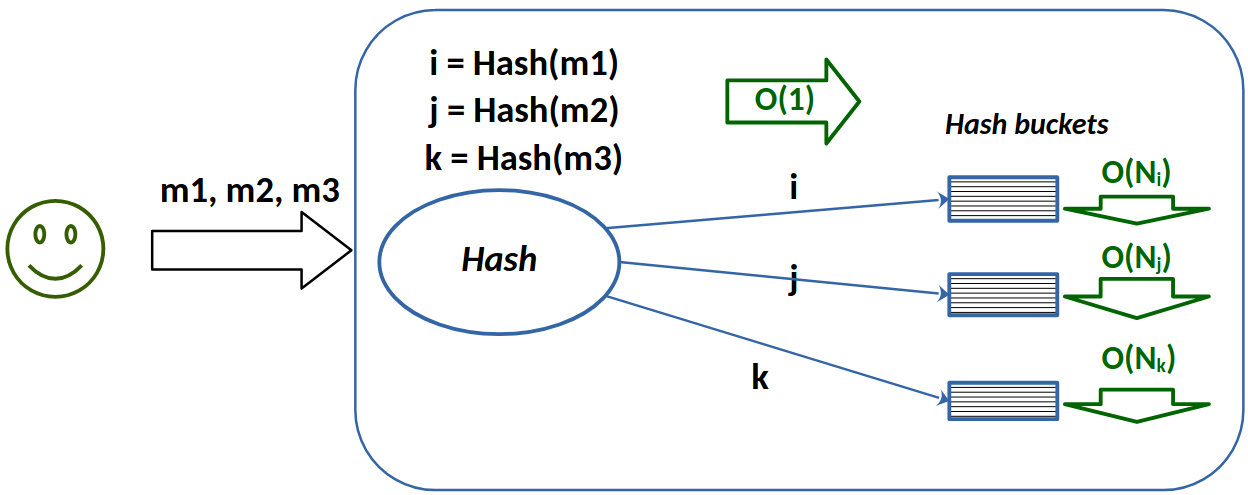
\includegraphics[width=\textwidth]{img/hc_dos.png}
        \end{minipage}
        \hfill
        \begin{minipage}[t]{0.45\textwidth}
            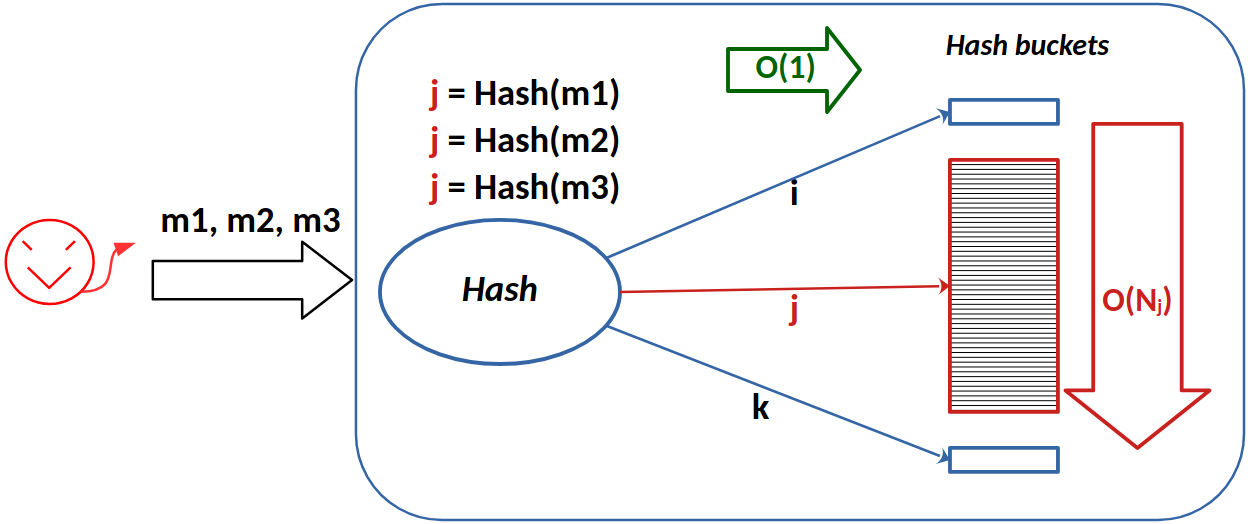
\includegraphics[width=\textwidth]{img/hc_dos_1.png}
            \centering
        \end{minipage}
    \end{figure}
    Anche nel caso in cui ci fosse un funzione hash crittografica, il costo dell'attacco sarebbe determinato dal \textbf{\textit{birthday attack}}, in più normalmente i \textit{bucket} hanno dimensione limitata, ad esempio $2^{16}$, mentre se utilizzasse una funzione hash crittografica i possibili valori, ad esempio di SHA256, sarebbe $2^{256}$ il che comunque non garantirebbe \textit{collision resistance} su un bucket. \\
    Se la struttura dati è esposta ad un attaccante potrebbe causare un \textbf{\textit{Denial of Service}} - un esempio possono essere i dizionari che vengono utilizzati per il \textit{routing} delle richieste web. Per mitigare questa casistica è possibile utilizzare un \textbf{\textit{Hash-based MAC}} - \textbf{HMAC} - dove il segreto viene scelto a \textit{runtime}. \textcolor{olive}{\textbf{vantaggi}}: per un avversario è praticamente impossibile trovare messaggi della tipologia definita in precedenza, \textcolor{red}{\textbf{svantaggi}}: le funzioni \textbf{MACs} sono molto più costose.
\end{flushleft}
\begin{boxA}
    \textcolor{red}{\textbf{\textit{SipHash}}} è una funzione \textbf{MAC} specializzata per \textit{tag} più piccoli - 64 bit. Pensata appositamente per casi d'uso del genere, ma non sicuro per la maggior parte dei contesti di comunicazione. La chiave non deve essere memorizzata, può essere cancellata nel momento in cui la tabella viene cancellata.
\end{boxA}

\section{Commitment Schemes}

\begin{flushleft}
    Uno \textbf{schema di \textit{commitment}} viene utilizzato per impedire ad un'entità di negare, in seguito, una certa scelta; possono essere utilizzati in maniera indipendenti o all'interno di altri protocolli. Un \textit{commitment scheme} deve avere due proprietà:
    \begin{enumerate}[nosep]
        \item \textbf{(obbligatorio) \textit{Binding}}: il \textit{commitment} è associato al valore scelto, non deve essere possibile fornire un valore diverso da quello iniziale che soddisfa la verifica.
        \item \textbf{(opzionale) \textit{Hiding}}: il \textit{commitment} deve nascondere il valore iniziale, deve essere garantita confidenzialità su ogni valore iniziale.
    \end{enumerate}

    Gli schemi di \textit{commitment} vengono utilizzati ad esempio: protocolli \textit{challenge-response} per l'autenticazione, alcuni schemi di firma digitale o autenticazione (\textbf{OAUTH PKCE}).

    \begin{figure}[h]
        \centering
        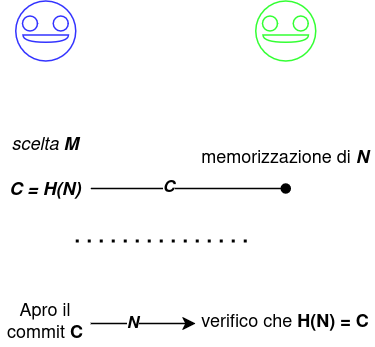
\includegraphics[width=0.35\textwidth]{img/commit_scheme.png}
    \end{figure}

    In questo caso viene utilizzata come funzione di commit una funzione \textbf{hash}, se questa rispetta la proprietà di \textit{collision resistance}, è possibile utilizzare anche una funzione \textbf{MAC}.
\end{flushleft}

\section{Authenticated Data Structure}

\begin{flushleft}
    Un'altra applicazione popolare per le funzioni hash sono gli schenari di \textbf{\textit{data outsourcing}} come precedentemente discusso per i \textit{web mirrors}. Vengono chiamati \textbf{\textit{authenticated data structure}} che è una versione estesa delle \textbf{strutture dati} - come ad esempio \textit{linked list}, \textit{binary tree} - alle quali vengono applicati i paradigmi di \textbf{integrità dei dati} mentre continuano a supportare \textbf{\textit{efficient queries}}.

    \begin{figure}[h]
        \centering
        \begin{minipage}[c]{0.45\textwidth}
            \centering
            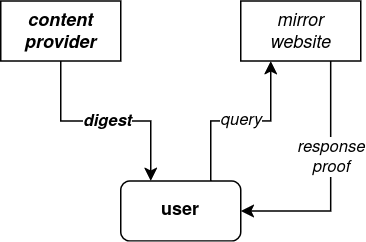
\includegraphics[width=\textwidth]{img/ads.png}
        \end{minipage}
        \hfill
        \begin{minipage}[c]{0.45\textwidth}
            \begin{enumerate}[nosep]
                \item download del \textit{digest}
                \item richiesta del dato
                \item risposta e prova
                \item l'utente accetta il dato se passa il controllo \textbf{verify(response, proof, digest)}
            \end{enumerate}
        \end{minipage}
    \end{figure}

    Analizziamo ora l'esempio di autenticazione di \textit{multiple data}, consideriamo un \textit{dataset} $\mathcal{X} = \{x_0, x_1, ..., x_n\}$, una possibilità per autenticare sarebbe quella di calcolarsi l'\textit{hash} di $\mathcal{X}$ ma questo vorrebbe dire calcolarsi $t = \text{HASH}(x_0 \; || \; x_1 \; || \; ... \; || \; x_n)$, in questo modo \textbf{verificare l'intergrità} di soltanto un dato avrebbe costo lineare in quanto bisognerebbe trasmettere tutti gli altri valori. \textbf{Soluzione: \textit{Merkle Hash Tree - MHT}}, dove gli hash vengono concatenati tramite un \textbf{albero binario}, le foglie sono gli hash dei valori di tutti i dati appartenenti al \textit{dataset}. L'inserimento e la validazione di un nuovo elemento costa $\mathcal{O}(\log n)$.

    \begin{figure}[h]
        \centering
        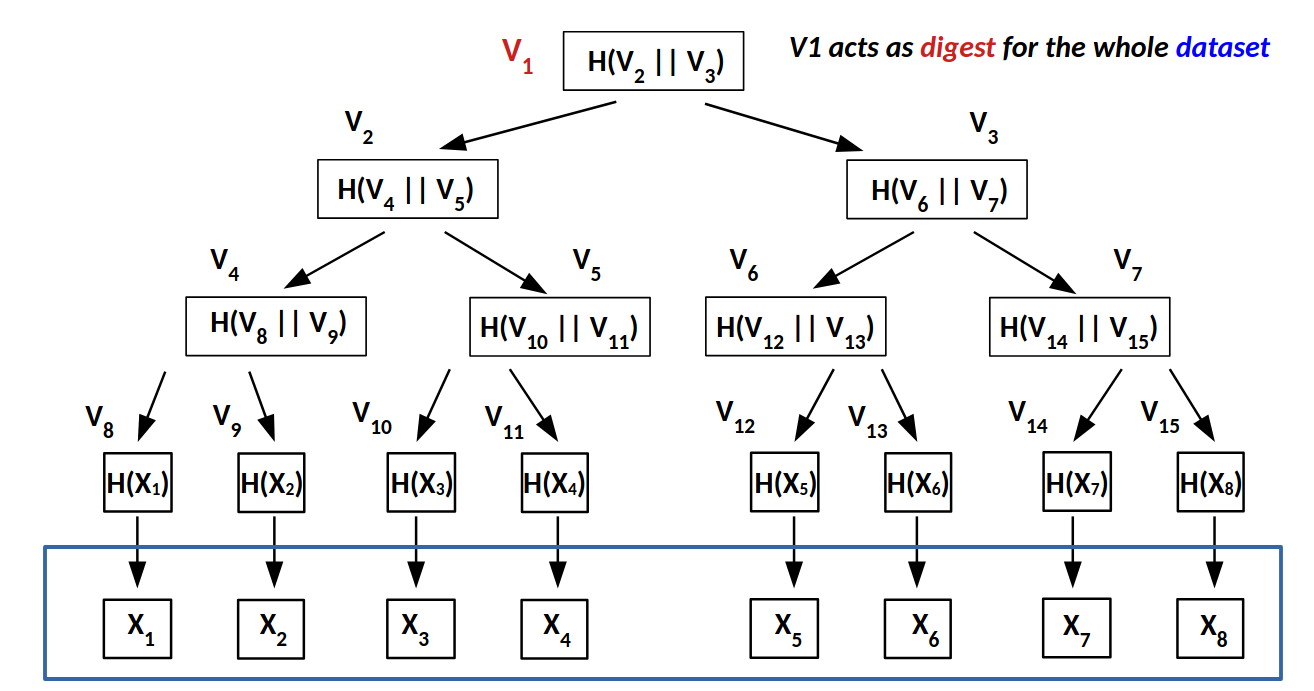
\includegraphics[width=\textwidth]{img/mht.png}
    \end{figure}

    Per validare - ad esempio - $x_3$, invece che dover inviare tutto il \textit{dataset} basterà inviare $x_3, v_{11}, v_4, v_3, v_1$ in questo modo si potrà calcolare $v_1 \overset{?}{=} h(\; h(\; h(\; h(x_3) \; || \; v_{11}) \; || \; v_4) \; || \; v_3)$, in questo modo si riesce a validare la appartenenza di un certo elemento al \textit{dataset}. \\
    A differenza della \textbf{\textit{membership proof}} di un elemento che è direttamente supportata in un \textbf{MHT}, la \textbf{\textit{non-membership proof}} non è supportata direttamente ma esistono modi per riuscirsela a ricavare:
    \begin{itemize}[nosep]
        \item \textbf{\textit{MHT} ordinato}: se gli elementi nei nodi della foglia sono ordinati si può provare che un elemento non è presente mostrando due \textbf{foglie adiacenti} $x_3, \; x_4$ tali che $x_3 < x < x_4$ e fornendo le \textbf{\textit{membership proof}} delle due foglie.
        \item \textbf{\textit{Sparse Merkle Tree}}: solitamente in un \textbf{SMT}, ogni possibile valore hash occupa una posizione predeterminata (tipicamente in base all'elemento), per dimostrare che $x$ \textbf{non esiste} si fornisce il cammino nel \textbf{SMT} dove dovrebbe trovarsi $x$ e si dimostra che è vuoto o continene un elemento $x' \neq x$.
    \end{itemize}
\end{flushleft}

\section{Synthetic Initialization Vectors}

\begin{flushleft}
    \textbf{SIV} denota una branchia di \textit{mode of operation} per gli schemi di crittografia autenticata che ha come scopo mitigare il danno che potrebbe fare il riuso di \textit{nonce} o dell'\textit{IV}. Il riuso di \textit{nonce} o \textit{IV} renderebbe lo schema \textbf{deterministico}, ma non perderebbe di sicurezza grazie a proprietà matematiche - nessun \textit{leak} di informazioni - a differenza di altri \textit{stream cipher} polinomiali tipo \textbf{GHASH} o \textbf{Poly1305}. ``\textbf{\textit{Synthetic}}'' in questo contesto significa che il \textit{nonce} o \textit{IV} forniti dall'utente non vengono utilizzati direttamente per cifrare, ma utilizzati per derivarne uno attraverso una funziona crittografica. In questo modo anche fornendo sempre lo stesso \textit{nonce} o \textit{IV} se il contenuto del messaggio cambia allora anche il \textbf{SIV} effettivo per cifrare cambierà.

    \begin{figure}[h]
        \centering
        \begin{minipage}[t]{0.45\textwidth}
            \centering
            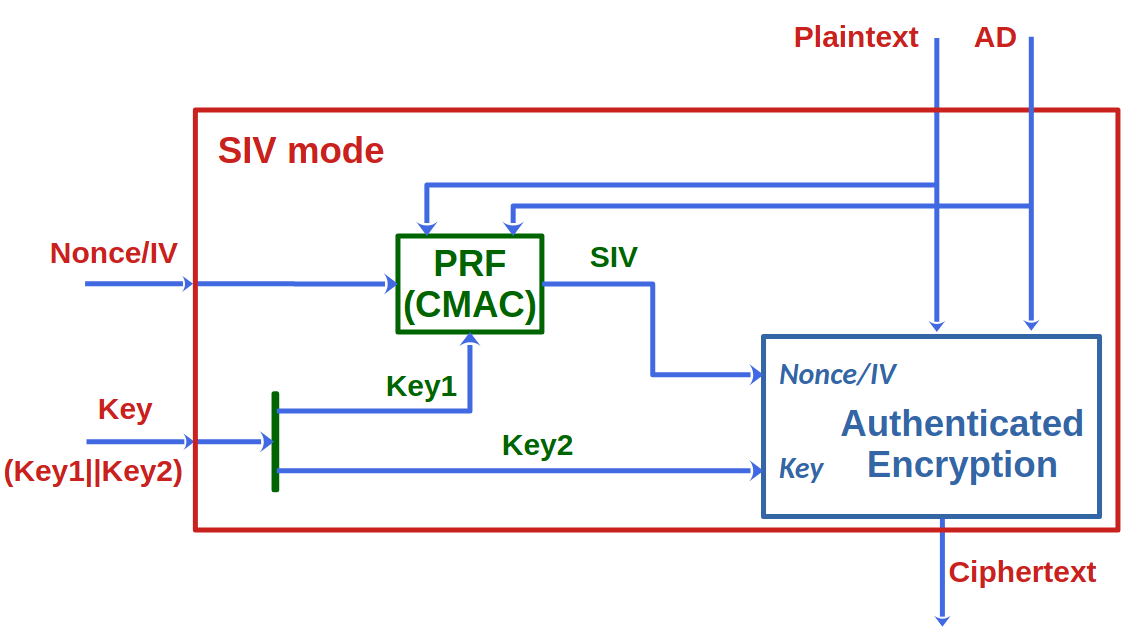
\includegraphics[width=\textwidth]{img/aes_siv.png}
            \caption{\textbf{\textit{AES-SIV}}}
        \end{minipage}
        \hfill
        \begin{minipage}[t]{0.45\textwidth}
            \centering
            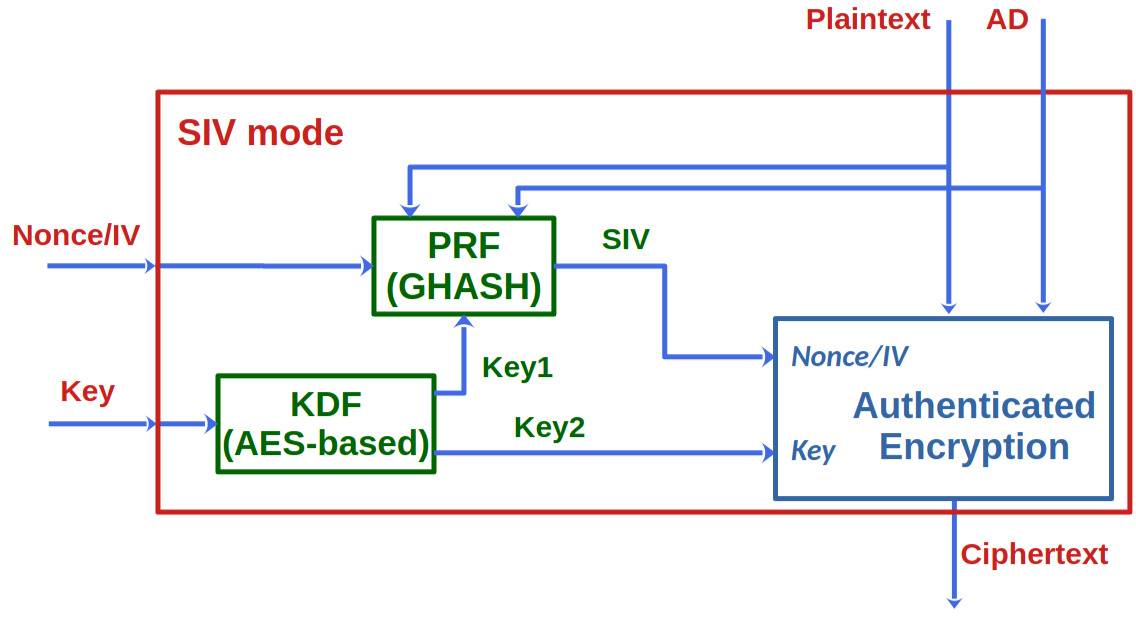
\includegraphics[width=\textwidth]{img/aes_gcm_siv.jpg}
            \caption{\textbf{\textit{AES-GCM-SIV}}}
        \end{minipage}
    \end{figure}
    Il maggior svantaggio di uno schema \textbf{SIV} è che la cifrazione del messaggio non può essere \textit{streamable}, infatti è necessario leggere il \textit{plaintext} deve essere letto due volte, la prima per generare il \textbf{SIV} (che dipende da tutto il testo in chiaro) e la seconda per l'algoritmo di \textit{encryption}, può essere un problema in caso di \textit{plaintext} molto grandi. Gli schemi \textbf{SIV} possono essere utilizzati per implementare \textcolor{red}{\textbf{\textit{Deterministic Encryption \& DEAED}}}.
\end{flushleft}

\section{(extra) Format-Preserving Encryption}